% Options for packages loaded elsewhere
\PassOptionsToPackage{unicode}{hyperref}
\PassOptionsToPackage{hyphens}{url}
%
\documentclass[
]{article}
\usepackage{amsmath,amssymb}
\usepackage{lmodern}
\usepackage{iftex}
\ifPDFTeX
  \usepackage[T1]{fontenc}
  \usepackage[utf8]{inputenc}
  \usepackage{textcomp} % provide euro and other symbols
\else % if luatex or xetex
  \usepackage{unicode-math}
  \defaultfontfeatures{Scale=MatchLowercase}
  \defaultfontfeatures[\rmfamily]{Ligatures=TeX,Scale=1}
\fi
% Use upquote if available, for straight quotes in verbatim environments
\IfFileExists{upquote.sty}{\usepackage{upquote}}{}
\IfFileExists{microtype.sty}{% use microtype if available
  \usepackage[]{microtype}
  \UseMicrotypeSet[protrusion]{basicmath} % disable protrusion for tt fonts
}{}
\makeatletter
\@ifundefined{KOMAClassName}{% if non-KOMA class
  \IfFileExists{parskip.sty}{%
    \usepackage{parskip}
  }{% else
    \setlength{\parindent}{0pt}
    \setlength{\parskip}{6pt plus 2pt minus 1pt}}
}{% if KOMA class
  \KOMAoptions{parskip=half}}
\makeatother
\usepackage{xcolor}
\usepackage[margin=1in]{geometry}
\usepackage{color}
\usepackage{fancyvrb}
\newcommand{\VerbBar}{|}
\newcommand{\VERB}{\Verb[commandchars=\\\{\}]}
\DefineVerbatimEnvironment{Highlighting}{Verbatim}{commandchars=\\\{\}}
% Add ',fontsize=\small' for more characters per line
\usepackage{framed}
\definecolor{shadecolor}{RGB}{248,248,248}
\newenvironment{Shaded}{\begin{snugshade}}{\end{snugshade}}
\newcommand{\AlertTok}[1]{\textcolor[rgb]{0.94,0.16,0.16}{#1}}
\newcommand{\AnnotationTok}[1]{\textcolor[rgb]{0.56,0.35,0.01}{\textbf{\textit{#1}}}}
\newcommand{\AttributeTok}[1]{\textcolor[rgb]{0.77,0.63,0.00}{#1}}
\newcommand{\BaseNTok}[1]{\textcolor[rgb]{0.00,0.00,0.81}{#1}}
\newcommand{\BuiltInTok}[1]{#1}
\newcommand{\CharTok}[1]{\textcolor[rgb]{0.31,0.60,0.02}{#1}}
\newcommand{\CommentTok}[1]{\textcolor[rgb]{0.56,0.35,0.01}{\textit{#1}}}
\newcommand{\CommentVarTok}[1]{\textcolor[rgb]{0.56,0.35,0.01}{\textbf{\textit{#1}}}}
\newcommand{\ConstantTok}[1]{\textcolor[rgb]{0.00,0.00,0.00}{#1}}
\newcommand{\ControlFlowTok}[1]{\textcolor[rgb]{0.13,0.29,0.53}{\textbf{#1}}}
\newcommand{\DataTypeTok}[1]{\textcolor[rgb]{0.13,0.29,0.53}{#1}}
\newcommand{\DecValTok}[1]{\textcolor[rgb]{0.00,0.00,0.81}{#1}}
\newcommand{\DocumentationTok}[1]{\textcolor[rgb]{0.56,0.35,0.01}{\textbf{\textit{#1}}}}
\newcommand{\ErrorTok}[1]{\textcolor[rgb]{0.64,0.00,0.00}{\textbf{#1}}}
\newcommand{\ExtensionTok}[1]{#1}
\newcommand{\FloatTok}[1]{\textcolor[rgb]{0.00,0.00,0.81}{#1}}
\newcommand{\FunctionTok}[1]{\textcolor[rgb]{0.00,0.00,0.00}{#1}}
\newcommand{\ImportTok}[1]{#1}
\newcommand{\InformationTok}[1]{\textcolor[rgb]{0.56,0.35,0.01}{\textbf{\textit{#1}}}}
\newcommand{\KeywordTok}[1]{\textcolor[rgb]{0.13,0.29,0.53}{\textbf{#1}}}
\newcommand{\NormalTok}[1]{#1}
\newcommand{\OperatorTok}[1]{\textcolor[rgb]{0.81,0.36,0.00}{\textbf{#1}}}
\newcommand{\OtherTok}[1]{\textcolor[rgb]{0.56,0.35,0.01}{#1}}
\newcommand{\PreprocessorTok}[1]{\textcolor[rgb]{0.56,0.35,0.01}{\textit{#1}}}
\newcommand{\RegionMarkerTok}[1]{#1}
\newcommand{\SpecialCharTok}[1]{\textcolor[rgb]{0.00,0.00,0.00}{#1}}
\newcommand{\SpecialStringTok}[1]{\textcolor[rgb]{0.31,0.60,0.02}{#1}}
\newcommand{\StringTok}[1]{\textcolor[rgb]{0.31,0.60,0.02}{#1}}
\newcommand{\VariableTok}[1]{\textcolor[rgb]{0.00,0.00,0.00}{#1}}
\newcommand{\VerbatimStringTok}[1]{\textcolor[rgb]{0.31,0.60,0.02}{#1}}
\newcommand{\WarningTok}[1]{\textcolor[rgb]{0.56,0.35,0.01}{\textbf{\textit{#1}}}}
\usepackage{longtable,booktabs,array}
\usepackage{calc} % for calculating minipage widths
% Correct order of tables after \paragraph or \subparagraph
\usepackage{etoolbox}
\makeatletter
\patchcmd\longtable{\par}{\if@noskipsec\mbox{}\fi\par}{}{}
\makeatother
% Allow footnotes in longtable head/foot
\IfFileExists{footnotehyper.sty}{\usepackage{footnotehyper}}{\usepackage{footnote}}
\makesavenoteenv{longtable}
\usepackage{graphicx}
\makeatletter
\def\maxwidth{\ifdim\Gin@nat@width>\linewidth\linewidth\else\Gin@nat@width\fi}
\def\maxheight{\ifdim\Gin@nat@height>\textheight\textheight\else\Gin@nat@height\fi}
\makeatother
% Scale images if necessary, so that they will not overflow the page
% margins by default, and it is still possible to overwrite the defaults
% using explicit options in \includegraphics[width, height, ...]{}
\setkeys{Gin}{width=\maxwidth,height=\maxheight,keepaspectratio}
% Set default figure placement to htbp
\makeatletter
\def\fps@figure{htbp}
\makeatother
\setlength{\emergencystretch}{3em} % prevent overfull lines
\providecommand{\tightlist}{%
  \setlength{\itemsep}{0pt}\setlength{\parskip}{0pt}}
\setcounter{secnumdepth}{-\maxdimen} % remove section numbering
\ifLuaTeX
  \usepackage{selnolig}  % disable illegal ligatures
\fi
\IfFileExists{bookmark.sty}{\usepackage{bookmark}}{\usepackage{hyperref}}
\IfFileExists{xurl.sty}{\usepackage{xurl}}{} % add URL line breaks if available
\urlstyle{same} % disable monospaced font for URLs
\hypersetup{
  pdftitle={JB Baseline - Reefs},
  pdfauthor={Molly Wilson},
  hidelinks,
  pdfcreator={LaTeX via pandoc}}

\title{JB Baseline - Reefs}
\author{Molly Wilson}
\date{8/14/2022}

\begin{document}
\maketitle

\hypertarget{section}{%
\section{}\label{section}}

\hypertarget{benthic}{%
\subsection{Benthic}\label{benthic}}

\begin{Shaded}
\begin{Highlighting}[]
\CommentTok{\# import and clean data}

\NormalTok{rf\_benthic }\OtherTok{\textless{}{-}} \FunctionTok{read\_excel}\NormalTok{(}\FunctionTok{here}\NormalTok{(}\StringTok{"jumby\_baseline"}\NormalTok{, }\StringTok{"data"}\NormalTok{, }\StringTok{"JBB\_reefs.xlsx"}\NormalTok{), }\AttributeTok{sheet =} \StringTok{"benthic"}\NormalTok{) }\SpecialCharTok{\%\textgreater{}\%}  
  \FunctionTok{clean\_names}\NormalTok{() }\SpecialCharTok{\%\textgreater{}\%}
  \FunctionTok{filter}\NormalTok{(}\SpecialCharTok{!}\FunctionTok{is.na}\NormalTok{(site)) }\SpecialCharTok{\%\textgreater{}\%} \CommentTok{\# remove any incomplete rows at the end of the data}
  \CommentTok{\# separate(species\_code, c("species\_code", "indicator")) \%\textgreater{}\% \# separating variables with an underscore into two columns}
  \FunctionTok{mutate}\NormalTok{(}\AttributeTok{species =} \FunctionTok{to\_any\_case}\NormalTok{(species, }\AttributeTok{case =} \StringTok{"sentence"}\NormalTok{), }\CommentTok{\# this makes sure species names are correctly capitalized}
         \CommentTok{\# site = to\_any\_case(site, case = "title"),}
         \CommentTok{\# consolidating categories here for graphs:}
         \AttributeTok{cat\_c =} \FunctionTok{case\_when}\NormalTok{(category\_code }\SpecialCharTok{\%in\%} \FunctionTok{c}\NormalTok{(}\StringTok{"LC"}\NormalTok{, }\StringTok{"SLC"}\NormalTok{) }\SpecialCharTok{\textasciitilde{}} \StringTok{"Hard corals"}\NormalTok{,}
\NormalTok{                                  category\_code }\SpecialCharTok{\%in\%} \FunctionTok{c}\NormalTok{(}\StringTok{"MA"}\NormalTok{) }\SpecialCharTok{\textasciitilde{}} \StringTok{"Macroalgae"}\NormalTok{,}
\NormalTok{                                  category\_code }\SpecialCharTok{\%in\%} \FunctionTok{c}\NormalTok{(}\StringTok{"TA"}\NormalTok{) }\SpecialCharTok{\textasciitilde{}} \StringTok{"Turf algae"}\NormalTok{,}
\NormalTok{                                  category\_code }\SpecialCharTok{\%in\%} \FunctionTok{c}\NormalTok{(}\StringTok{"CCA"}\NormalTok{, }\StringTok{"CCA\_ND"}\NormalTok{) }\SpecialCharTok{\textasciitilde{}} \StringTok{"CCA"}\NormalTok{,}
\NormalTok{                                  category\_code }\SpecialCharTok{\%in\%} \FunctionTok{c}\NormalTok{(}\StringTok{"OINV"}\NormalTok{, }\StringTok{"SPON"}\NormalTok{, }\StringTok{"AINV"}\NormalTok{, }\StringTok{"CYAN"}\NormalTok{, }\StringTok{"PEY"}\NormalTok{) }\SpecialCharTok{\textasciitilde{}} \StringTok{"Other competitors"}\NormalTok{,}
\NormalTok{                                  category\_code }\SpecialCharTok{\%in\%} \FunctionTok{c}\NormalTok{(}\StringTok{"SAND"}\NormalTok{, }\StringTok{"HOLE"}\NormalTok{, }\StringTok{"SG"}\NormalTok{, }\StringTok{"PAVE"}\NormalTok{) }\SpecialCharTok{\textasciitilde{}} \StringTok{"Other substratum"}
\NormalTok{                                    ),}
         \CommentTok{\# adding algal type for graphs about palatability:}
         \AttributeTok{algal\_type =} \FunctionTok{case\_when}\NormalTok{(type\_code }\SpecialCharTok{\%in\%} \FunctionTok{c}\NormalTok{(}\StringTok{"BFMA"}\NormalTok{, }\StringTok{"GFMA"}\NormalTok{, }\StringTok{"RFMA"}\NormalTok{) }\SpecialCharTok{\textasciitilde{}} \StringTok{"Fleshy macroalgae"}\NormalTok{,}
\NormalTok{                                type\_code }\SpecialCharTok{\%in\%} \FunctionTok{c}\NormalTok{(}\StringTok{"GCMA"}\NormalTok{, }\StringTok{"RCMA"}\NormalTok{) }\SpecialCharTok{\textasciitilde{}} \StringTok{"Calcareous macroalgae"}\NormalTok{,}
\NormalTok{                                type\_code }\SpecialCharTok{\%in\%} \FunctionTok{c}\NormalTok{(}\StringTok{"TA"}\NormalTok{, }\StringTok{"TAS"}\NormalTok{, }\StringTok{"STA"}\NormalTok{) }\SpecialCharTok{\textasciitilde{}} \StringTok{"Turf algae"}\NormalTok{),}
         \CommentTok{\# certain substrates are not suitable for coral or algal growth, so should not detract from percent cover}
         \AttributeTok{av\_sub\_yn =} \FunctionTok{if\_else}\NormalTok{(category\_code }\SpecialCharTok{\%in\%} \FunctionTok{c}\NormalTok{(}\StringTok{"SAND"}\NormalTok{, }\StringTok{"HOLE"}\NormalTok{, }\StringTok{"SG"}\NormalTok{, }\StringTok{"PAVE"}\NormalTok{), }\StringTok{"no"}\NormalTok{, }\StringTok{"yes"}\NormalTok{)}
\NormalTok{         ) }\SpecialCharTok{\%\textgreater{}\%}
    \FunctionTok{filter}\NormalTok{(}\SpecialCharTok{!}\FunctionTok{is.na}\NormalTok{(cat\_c) }\SpecialCharTok{\&} \SpecialCharTok{!}\FunctionTok{is.na}\NormalTok{(species)) }\CommentTok{\# need GRB to fix some data errors, but using this for now}
\end{Highlighting}
\end{Shaded}

\hypertarget{percent-cover}{%
\subsubsection{Percent cover}\label{percent-cover}}

\hypertarget{percent-cover-by-site-and-category}{%
\paragraph{Percent cover by site and
category}\label{percent-cover-by-site-and-category}}

\begin{Shaded}
\begin{Highlighting}[]
\CommentTok{\# "expand" dataframe so that it contains all benthic categories per site/transect/meter {-}\textgreater{} join full dataset so that any meters where a species was absent it will show up as 0 (as opposed to having no entry)}
\NormalTok{rf\_pc\_cat\_m }\OtherTok{\textless{}{-}}\NormalTok{ rf\_benthic }\SpecialCharTok{\%\textgreater{}\%}
  \FunctionTok{filter}\NormalTok{(av\_sub\_yn }\SpecialCharTok{==} \StringTok{"yes"}\NormalTok{) }\SpecialCharTok{\%\textgreater{}\%} \CommentTok{\# percent cover is relative to available substrate}
  \FunctionTok{expand}\NormalTok{(}\FunctionTok{nesting}\NormalTok{(site, transect, meter), cat\_c) }\SpecialCharTok{\%\textgreater{}\%}
  \CommentTok{\# this is where we add in our actual data to this expanded template:}
  \FunctionTok{left\_join}\NormalTok{(rf\_benthic }\SpecialCharTok{\%\textgreater{}\%} 
              \FunctionTok{filter}\NormalTok{(av\_sub\_yn }\SpecialCharTok{==} \StringTok{"yes"}\NormalTok{) }\SpecialCharTok{\%\textgreater{}\%} \CommentTok{\# only looking at what is considered available substrate (no sand, etc.)}
              \FunctionTok{group\_by}\NormalTok{(site, transect, meter) }\SpecialCharTok{\%\textgreater{}\%}
              \FunctionTok{mutate}\NormalTok{(}\AttributeTok{n\_pts =} \FunctionTok{n}\NormalTok{()) }\SpecialCharTok{\%\textgreater{}\%} \CommentTok{\# showing total number of points per meter that are considered available substrate}
              \FunctionTok{ungroup}\NormalTok{() }\SpecialCharTok{\%\textgreater{}\%}
              \FunctionTok{group\_by}\NormalTok{(site, transect, meter, n\_pts, cat\_c) }\SpecialCharTok{\%\textgreater{}\%}
              \FunctionTok{summarize}\NormalTok{(}\AttributeTok{pc\_m =} \DecValTok{100}\SpecialCharTok{*}\FunctionTok{n}\NormalTok{()}\SpecialCharTok{/}\NormalTok{n\_pts) }\SpecialCharTok{\%\textgreater{}\%} \CommentTok{\# n() counts the number of entries within a given group}
              \FunctionTok{ungroup}\NormalTok{() }\SpecialCharTok{\%\textgreater{}\%}
              \FunctionTok{distinct}\NormalTok{() }\SpecialCharTok{\%\textgreater{}\%}
              \FunctionTok{select}\NormalTok{(}\SpecialCharTok{{-}}\NormalTok{n\_pts), }
            \AttributeTok{by =} \FunctionTok{c}\NormalTok{(}\StringTok{"site"}\NormalTok{, }\StringTok{"transect"}\NormalTok{, }\StringTok{"meter"}\NormalTok{, }\StringTok{"cat\_c"}\NormalTok{)) }\SpecialCharTok{\%\textgreater{}\%}
  \FunctionTok{mutate}\NormalTok{(}\AttributeTok{pc\_m =} \FunctionTok{if\_else}\NormalTok{(}\FunctionTok{is.na}\NormalTok{(pc\_m), }\DecValTok{0}\NormalTok{, pc\_m))}

\CommentTok{\# average these meter{-}level results within transect, then within sites}
\NormalTok{rf\_pc\_cat\_site }\OtherTok{\textless{}{-}}\NormalTok{ rf\_pc\_cat\_m }\SpecialCharTok{\%\textgreater{}\%}
  \FunctionTok{group\_by}\NormalTok{(site, transect, cat\_c) }\SpecialCharTok{\%\textgreater{}\%}
  \FunctionTok{summarize}\NormalTok{(}\AttributeTok{pc\_t =} \FunctionTok{mean}\NormalTok{(pc\_m)) }\SpecialCharTok{\%\textgreater{}\%}
  \FunctionTok{ungroup}\NormalTok{() }\SpecialCharTok{\%\textgreater{}\%}
  \FunctionTok{group\_by}\NormalTok{(site, cat\_c) }\SpecialCharTok{\%\textgreater{}\%}
  \FunctionTok{summarize}\NormalTok{(}\AttributeTok{n\_test =} \FunctionTok{n}\NormalTok{(),}
            \AttributeTok{pc\_mean =} \FunctionTok{mean}\NormalTok{(pc\_t),}
            \AttributeTok{pc\_se =} \FunctionTok{sd}\NormalTok{(pc\_t)}\SpecialCharTok{/}\FunctionTok{sqrt}\NormalTok{(}\FunctionTok{n}\NormalTok{())}
\NormalTok{            ) }\SpecialCharTok{\%\textgreater{}\%}
  \FunctionTok{filter}\NormalTok{(cat\_c }\SpecialCharTok{!=} \StringTok{"Other substratum"}\NormalTok{) }\SpecialCharTok{\%\textgreater{}\%} 
  \FunctionTok{mutate}\NormalTok{(}\AttributeTok{cat\_c =} \FunctionTok{factor}\NormalTok{(cat\_c, }\AttributeTok{levels =} \FunctionTok{c}\NormalTok{(}\StringTok{"Hard corals"}\NormalTok{, }\StringTok{"CCA"}\NormalTok{, }\StringTok{"Macroalgae"}\NormalTok{, }\StringTok{"Turf algae"}\NormalTok{, }\StringTok{"Other competitors"}\NormalTok{)))}

\CommentTok{\# quick check to make sure everything adds up to 100\% at the meter and site level}
\NormalTok{test1 }\OtherTok{\textless{}{-}}\NormalTok{ rf\_pc\_cat\_m }\SpecialCharTok{\%\textgreater{}\%}
  \FunctionTok{group\_by}\NormalTok{(site, transect, meter) }\SpecialCharTok{\%\textgreater{}\%}
  \FunctionTok{summarize}\NormalTok{(}\AttributeTok{total =} \FunctionTok{sum}\NormalTok{(pc\_m))}
\NormalTok{test2 }\OtherTok{\textless{}{-}}\NormalTok{ rf\_pc\_cat\_site }\SpecialCharTok{\%\textgreater{}\%}
  \FunctionTok{group\_by}\NormalTok{(site) }\SpecialCharTok{\%\textgreater{}\%}
  \FunctionTok{summarize}\NormalTok{(}\AttributeTok{total =} \FunctionTok{sum}\NormalTok{(pc\_mean))}
\end{Highlighting}
\end{Shaded}

\begin{Shaded}
\begin{Highlighting}[]
\NormalTok{cat\_palette }\OtherTok{\textless{}{-}} \FunctionTok{c}\NormalTok{(}\StringTok{"coral2"}\NormalTok{, }\StringTok{"pink"}\NormalTok{, }\StringTok{"darkolivegreen"}\NormalTok{, }\StringTok{"darkkhaki"}\NormalTok{, }\StringTok{"slategray3"}\NormalTok{)}
\FunctionTok{ggplot}\NormalTok{(rf\_pc\_cat\_site, }
       \FunctionTok{aes}\NormalTok{(}\AttributeTok{x =}\NormalTok{ cat\_c, }\AttributeTok{y =}\NormalTok{ pc\_mean, }\AttributeTok{fill =}\NormalTok{ cat\_c)) }\SpecialCharTok{+}
  \FunctionTok{geom\_col}\NormalTok{(}\AttributeTok{color =} \StringTok{"black"}\NormalTok{, }\AttributeTok{alpha =} \FloatTok{0.9}\NormalTok{) }\SpecialCharTok{+}
  \FunctionTok{geom\_errorbar}\NormalTok{(}\FunctionTok{aes}\NormalTok{(}\AttributeTok{ymin =}\NormalTok{ pc\_mean }\SpecialCharTok{{-}}\NormalTok{ pc\_se, }\AttributeTok{ymax =}\NormalTok{ pc\_mean }\SpecialCharTok{+}\NormalTok{ pc\_se), }\AttributeTok{width =}\NormalTok{ .}\DecValTok{2}\NormalTok{,}
                 \AttributeTok{position =} \FunctionTok{position\_dodge}\NormalTok{(.}\DecValTok{9}\NormalTok{)) }\SpecialCharTok{+}
  \FunctionTok{scale\_fill\_manual}\NormalTok{(}\AttributeTok{values =}\NormalTok{ cat\_palette) }\SpecialCharTok{+}
  \FunctionTok{facet\_wrap}\NormalTok{(. }\SpecialCharTok{\textasciitilde{}}\NormalTok{ site, }\AttributeTok{ncol =} \DecValTok{2}\NormalTok{) }\SpecialCharTok{+}
  \FunctionTok{labs}\NormalTok{(}\AttributeTok{y =} \StringTok{"Mean percent cover"}\NormalTok{, }\AttributeTok{x =} \StringTok{""}\NormalTok{, }\AttributeTok{fill =} \StringTok{""}\NormalTok{) }\SpecialCharTok{+}
  \FunctionTok{theme\_bw}\NormalTok{() }\SpecialCharTok{+}
  \FunctionTok{theme}\NormalTok{(}\AttributeTok{axis.text.x =} \FunctionTok{element\_text}\NormalTok{(}\AttributeTok{angle =} \DecValTok{45}\NormalTok{, }\AttributeTok{h =} \DecValTok{1}\NormalTok{, }\AttributeTok{face =} \StringTok{"italic"}\NormalTok{))}
\end{Highlighting}
\end{Shaded}

\begin{Shaded}
\begin{Highlighting}[]
\NormalTok{cat\_palette }\OtherTok{\textless{}{-}} \FunctionTok{c}\NormalTok{(}\StringTok{"coral2"}\NormalTok{, }\StringTok{"pink"}\NormalTok{, }\StringTok{"darkolivegreen"}\NormalTok{, }\StringTok{"darkkhaki"}\NormalTok{, }\StringTok{"slategray3"}\NormalTok{)}
\FunctionTok{ggplot}\NormalTok{(rf\_pc\_cat\_site, }
       \FunctionTok{aes}\NormalTok{(}\AttributeTok{x =} \StringTok{"cat\_c"}\NormalTok{, }\AttributeTok{y =}\NormalTok{ pc\_mean, }\AttributeTok{fill =}\NormalTok{ cat\_c)) }\SpecialCharTok{+} 
  \FunctionTok{geom\_bar}\NormalTok{(}\AttributeTok{width =} \DecValTok{1}\NormalTok{, }\AttributeTok{stat =} \StringTok{"identity"}\NormalTok{, }\AttributeTok{color =} \StringTok{"black"}\NormalTok{) }\SpecialCharTok{+}
  \FunctionTok{coord\_polar}\NormalTok{(}\StringTok{"y"}\NormalTok{, }\AttributeTok{start=}\DecValTok{0}\NormalTok{) }\SpecialCharTok{+}
  \FunctionTok{scale\_fill\_manual}\NormalTok{(}\AttributeTok{values =}\NormalTok{ cat\_palette) }\SpecialCharTok{+}
  \FunctionTok{facet\_wrap}\NormalTok{(}\FunctionTok{vars}\NormalTok{(site), }\AttributeTok{nrow =} \DecValTok{2}\NormalTok{) }\SpecialCharTok{+}
  \FunctionTok{theme\_void}\NormalTok{() }\SpecialCharTok{+}
  \FunctionTok{theme}\NormalTok{(}\AttributeTok{legend.position =} \StringTok{"bottom"}\NormalTok{,}
        \AttributeTok{legend.title =} \FunctionTok{element\_blank}\NormalTok{(),}
        \AttributeTok{panel.spacing =} \FunctionTok{unit}\NormalTok{(}\DecValTok{1}\NormalTok{, }\StringTok{"lines"}\NormalTok{))}
\end{Highlighting}
\end{Shaded}

\includegraphics{jbb_reefs_files/figure-latex/unnamed-chunk-5-1.pdf}

\begin{Shaded}
\begin{Highlighting}[]
\FunctionTok{kable}\NormalTok{(rf\_pc\_cat\_site }\SpecialCharTok{\%\textgreater{}\%} \FunctionTok{select}\NormalTok{(site, }\AttributeTok{category =}\NormalTok{ cat\_c, pc\_mean, pc\_se))}
\end{Highlighting}
\end{Shaded}

\begin{longtable}[]{@{}llrr@{}}
\toprule()
site & category & pc\_mean & pc\_se \\
\midrule()
\endhead
Homer Point & CCA & 14.500000 & 3.5000000 \\
Homer Point & Hard corals & 12.500000 & 7.5000000 \\
Homer Point & Macroalgae & 20.000000 & 15.0000000 \\
Homer Point & Other competitors & 22.000000 & 7.0000000 \\
Homer Point & Turf algae & 31.000000 & 4.0000000 \\
Little Bird Island N & CCA & 24.000000 & 5.1316014 \\
Little Bird Island N & Hard corals & 18.000000 & 2.0816660 \\
Little Bird Island N & Macroalgae & 16.333333 & 4.0551750 \\
Little Bird Island N & Other competitors & 13.333333 & 0.6666667 \\
Little Bird Island N & Turf algae & 28.333333 & 4.9103066 \\
Little Bird Island W & CCA & 9.037037 & 1.7642230 \\
Little Bird Island W & Hard corals & 62.148148 & 7.9572762 \\
Little Bird Island W & Macroalgae & 6.000000 & 4.5825757 \\
Little Bird Island W & Other competitors & 5.666667 & 1.2018504 \\
Little Bird Island W & Turf algae & 17.148148 & 5.0537577 \\
Pasture Point & CCA & 21.111111 & 5.8888889 \\
Pasture Point & Hard corals & 12.277778 & 1.2777778 \\
Pasture Point & Macroalgae & 21.722222 & 3.7222222 \\
Pasture Point & Other competitors & 11.555556 & 3.4444444 \\
Pasture Point & Turf algae & 33.333333 & 4.3333333 \\
Pierce Shoals W & CCA & 35.666667 & 8.0897741 \\
Pierce Shoals W & Hard corals & 20.000000 & 7.8102497 \\
Pierce Shoals W & Macroalgae & 0.000000 & 0.0000000 \\
Pierce Shoals W & Other competitors & 7.666667 & 2.4037009 \\
Pierce Shoals W & Turf algae & 36.666667 & 3.1797973 \\
\bottomrule()
\end{longtable}

\hypertarget{percent-cover-by-species}{%
\subsubsection{Percent cover by
species}\label{percent-cover-by-species}}

\begin{Shaded}
\begin{Highlighting}[]
\CommentTok{\# calculating percent cover by species at each meter}
\NormalTok{rf\_pc\_spp\_m }\OtherTok{\textless{}{-}}\NormalTok{ rf\_benthic }\SpecialCharTok{\%\textgreater{}\%}
  \FunctionTok{filter}\NormalTok{(av\_sub\_yn }\SpecialCharTok{==} \StringTok{"yes"}\NormalTok{) }\SpecialCharTok{\%\textgreater{}\%}
  \FunctionTok{expand}\NormalTok{(}\FunctionTok{nesting}\NormalTok{(site, transect, meter), }\FunctionTok{nesting}\NormalTok{(species, cat\_c)) }\SpecialCharTok{\%\textgreater{}\%}
  \FunctionTok{left\_join}\NormalTok{(rf\_benthic }\SpecialCharTok{\%\textgreater{}\%} 
              \FunctionTok{filter}\NormalTok{(av\_sub\_yn }\SpecialCharTok{==} \StringTok{"yes"}\NormalTok{) }\SpecialCharTok{\%\textgreater{}\%} 
              \FunctionTok{group\_by}\NormalTok{(site, transect, meter) }\SpecialCharTok{\%\textgreater{}\%}
              \FunctionTok{mutate}\NormalTok{(}\AttributeTok{n\_pts =} \FunctionTok{n}\NormalTok{()) }\SpecialCharTok{\%\textgreater{}\%} 
              \FunctionTok{ungroup}\NormalTok{() }\SpecialCharTok{\%\textgreater{}\%}
              \FunctionTok{group\_by}\NormalTok{(site, transect, meter, n\_pts, species, cat\_c) }\SpecialCharTok{\%\textgreater{}\%}
              \FunctionTok{summarize}\NormalTok{(}\AttributeTok{pc\_m =} \DecValTok{100}\SpecialCharTok{*}\FunctionTok{n}\NormalTok{()}\SpecialCharTok{/}\NormalTok{n\_pts) }\SpecialCharTok{\%\textgreater{}\%}
              \FunctionTok{ungroup}\NormalTok{() }\SpecialCharTok{\%\textgreater{}\%}
              \FunctionTok{distinct}\NormalTok{() }\SpecialCharTok{\%\textgreater{}\%}
              \FunctionTok{select}\NormalTok{(}\SpecialCharTok{{-}}\NormalTok{n\_pts), }
            \AttributeTok{by =} \FunctionTok{c}\NormalTok{(}\StringTok{"site"}\NormalTok{, }\StringTok{"transect"}\NormalTok{, }\StringTok{"meter"}\NormalTok{, }\StringTok{"species"}\NormalTok{, }\StringTok{"cat\_c"}\NormalTok{)) }\SpecialCharTok{\%\textgreater{}\%}
  \FunctionTok{mutate}\NormalTok{(}\AttributeTok{pc\_m =} \FunctionTok{if\_else}\NormalTok{(}\FunctionTok{is.na}\NormalTok{(pc\_m), }\DecValTok{0}\NormalTok{, pc\_m))}

\CommentTok{\# calculating mean percent cover by transect {-}\textgreater{} site}
\NormalTok{rf\_pc\_spp\_site }\OtherTok{\textless{}{-}}\NormalTok{ rf\_pc\_spp\_m }\SpecialCharTok{\%\textgreater{}\%}
  \FunctionTok{group\_by}\NormalTok{(site, transect, species, cat\_c) }\SpecialCharTok{\%\textgreater{}\%}
  \FunctionTok{summarize}\NormalTok{(}\AttributeTok{pc\_t =} \FunctionTok{mean}\NormalTok{(pc\_m)) }\SpecialCharTok{\%\textgreater{}\%}
  \FunctionTok{ungroup}\NormalTok{() }\SpecialCharTok{\%\textgreater{}\%}
  \FunctionTok{group\_by}\NormalTok{(site, species, cat\_c) }\SpecialCharTok{\%\textgreater{}\%}
  \FunctionTok{summarize}\NormalTok{(}\AttributeTok{pc\_mean =} \FunctionTok{mean}\NormalTok{(pc\_t),}
            \AttributeTok{pc\_se =} \FunctionTok{sd}\NormalTok{(pc\_t)}\SpecialCharTok{/}\FunctionTok{sqrt}\NormalTok{(}\FunctionTok{n}\NormalTok{())}
\NormalTok{            ) }\SpecialCharTok{\%\textgreater{}\%}
  \FunctionTok{ungroup}\NormalTok{() }\SpecialCharTok{\%\textgreater{}\%}
  \FunctionTok{distinct}\NormalTok{()}

\CommentTok{\# calculating mean percent cover by species across all sites}
\NormalTok{rf\_pc\_spp }\OtherTok{\textless{}{-}}\NormalTok{ rf\_pc\_spp\_site }\SpecialCharTok{\%\textgreater{}\%}
  \FunctionTok{group\_by}\NormalTok{(species, cat\_c) }\SpecialCharTok{\%\textgreater{}\%}
  \FunctionTok{summarize}\NormalTok{(}\AttributeTok{pc =} \FunctionTok{mean}\NormalTok{(pc\_mean),}
            \AttributeTok{pc\_se =} \FunctionTok{sd}\NormalTok{(pc\_mean)}\SpecialCharTok{/}\FunctionTok{sqrt}\NormalTok{(}\FunctionTok{n}\NormalTok{())) }\SpecialCharTok{\%\textgreater{}\%}
  \FunctionTok{rename}\NormalTok{(}\AttributeTok{pc\_mean =}\NormalTok{ pc) }

\CommentTok{\# testing that total percent cover per transect and site add up to 100}
\NormalTok{test1 }\OtherTok{\textless{}{-}}\NormalTok{ rf\_pc\_spp\_m }\SpecialCharTok{\%\textgreater{}\%}
  \FunctionTok{group\_by}\NormalTok{(site, transect, meter) }\SpecialCharTok{\%\textgreater{}\%}
  \FunctionTok{summarize}\NormalTok{(}\AttributeTok{total =} \FunctionTok{sum}\NormalTok{(pc\_m))}
\NormalTok{test2 }\OtherTok{\textless{}{-}}\NormalTok{ rf\_pc\_spp\_site }\SpecialCharTok{\%\textgreater{}\%}
  \FunctionTok{group\_by}\NormalTok{(site) }\SpecialCharTok{\%\textgreater{}\%}
  \FunctionTok{summarize}\NormalTok{(}\AttributeTok{total =} \FunctionTok{sum}\NormalTok{(pc\_mean))}
\NormalTok{test3 }\OtherTok{\textless{}{-}} \FunctionTok{sum}\NormalTok{(rf\_pc\_spp}\SpecialCharTok{$}\NormalTok{pc\_mean)}
\end{Highlighting}
\end{Shaded}

\hypertarget{stony-coral---percent-cover-by-species-across-all-sites}{%
\paragraph{Stony coral - percent cover by species across all
sites}\label{stony-coral---percent-cover-by-species-across-all-sites}}

\begin{Shaded}
\begin{Highlighting}[]
\FunctionTok{ggplot}\NormalTok{(rf\_pc\_spp }\SpecialCharTok{\%\textgreater{}\%}
         \FunctionTok{filter}\NormalTok{(cat\_c }\SpecialCharTok{==} \StringTok{"Hard corals"}\NormalTok{),}
       \FunctionTok{aes}\NormalTok{(}\AttributeTok{x =} \FunctionTok{reorder}\NormalTok{(species, pc\_mean), }\AttributeTok{y =}\NormalTok{ pc\_mean)) }\SpecialCharTok{+}
  \FunctionTok{geom\_col}\NormalTok{(}\AttributeTok{fill =} \StringTok{"coral2"}\NormalTok{, }\AttributeTok{color =} \StringTok{"black"}\NormalTok{, }\AttributeTok{alpha =} \FloatTok{0.9}\NormalTok{) }\SpecialCharTok{+}
  \FunctionTok{geom\_errorbar}\NormalTok{(}\FunctionTok{aes}\NormalTok{(}\AttributeTok{ymin =}\NormalTok{ pc\_mean }\SpecialCharTok{{-}}\NormalTok{ pc\_se, }\AttributeTok{ymax =}\NormalTok{ pc\_mean }\SpecialCharTok{+}\NormalTok{ pc\_se), }\AttributeTok{width =}\NormalTok{ .}\DecValTok{2}\NormalTok{,}
                 \AttributeTok{position =} \FunctionTok{position\_dodge}\NormalTok{(.}\DecValTok{9}\NormalTok{)) }\SpecialCharTok{+}
  \FunctionTok{coord\_flip}\NormalTok{() }\SpecialCharTok{+}
  \FunctionTok{labs}\NormalTok{(}\AttributeTok{y =} \StringTok{"Mean percent cover"}\NormalTok{, }\AttributeTok{x =} \StringTok{""}\NormalTok{, }\AttributeTok{fill =} \StringTok{""}\NormalTok{) }\SpecialCharTok{+}
  \FunctionTok{theme\_bw}\NormalTok{() }\SpecialCharTok{+}
  \FunctionTok{theme}\NormalTok{(}\AttributeTok{axis.text.y =} \FunctionTok{element\_text}\NormalTok{(}\AttributeTok{face =} \StringTok{"italic"}\NormalTok{))}
\end{Highlighting}
\end{Shaded}

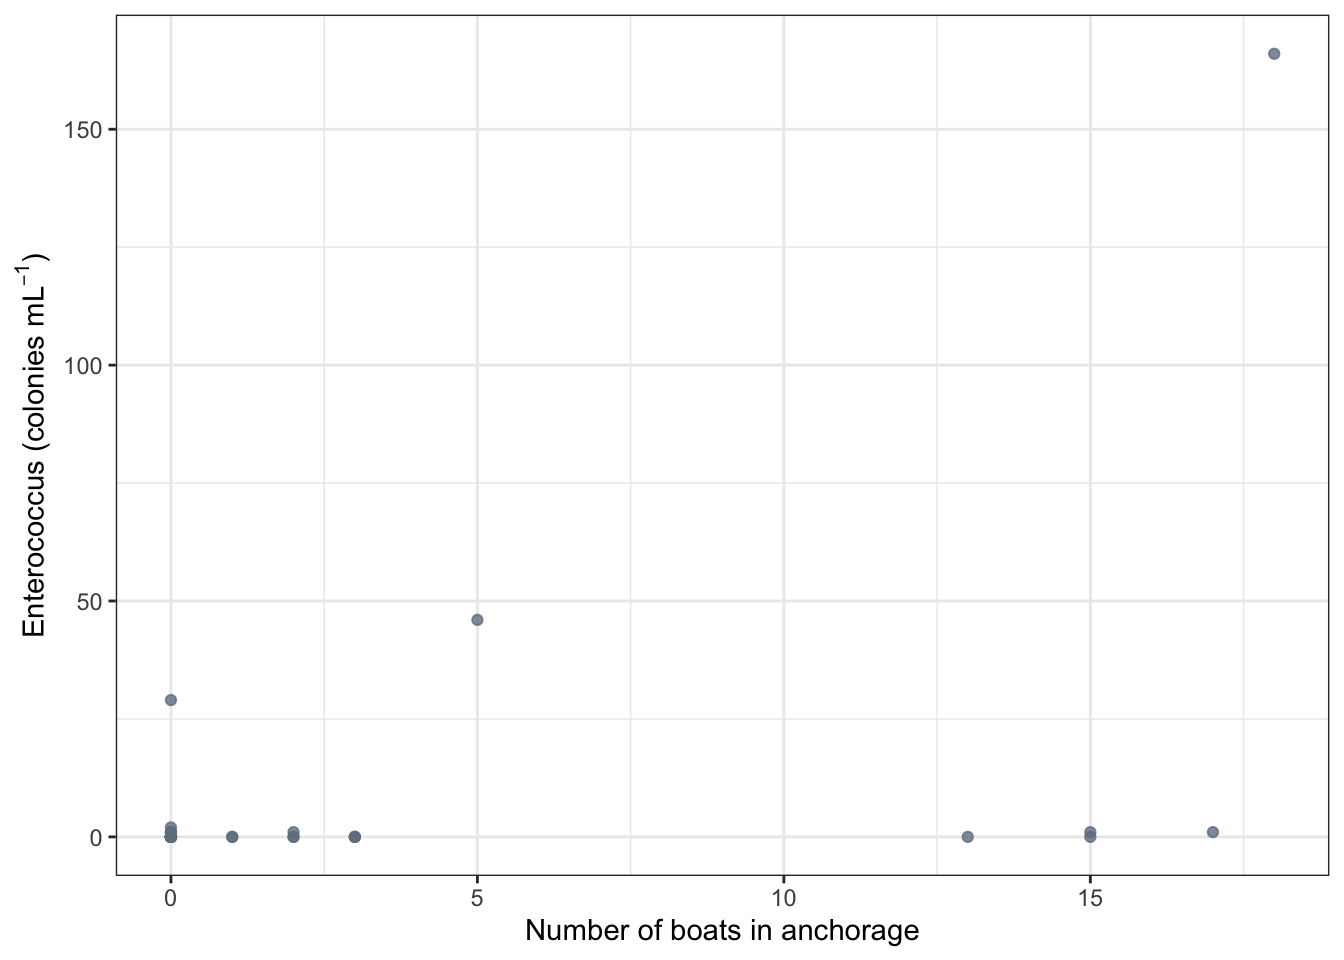
\includegraphics{jbb_reefs_files/figure-latex/unnamed-chunk-7-1.pdf}

\begin{Shaded}
\begin{Highlighting}[]
\FunctionTok{kable}\NormalTok{(rf\_pc\_spp }\SpecialCharTok{\%\textgreater{}\%} \FunctionTok{filter}\NormalTok{(cat\_c }\SpecialCharTok{==} \StringTok{"Hard corals"}\NormalTok{) }\SpecialCharTok{\%\textgreater{}\%} \FunctionTok{select}\NormalTok{(species, pc\_mean, pc\_se))}
\end{Highlighting}
\end{Shaded}

\begin{longtable}[]{@{}lrr@{}}
\toprule()
species & pc\_mean & pc\_se \\
\midrule()
\endhead
Acropora cervicornis & 2.1777778 & 2.1777778 \\
Acropora palmata & 4.0000000 & 1.8287822 \\
Acropora prolifera & 9.7000000 & 6.3000000 \\
Agaricia agaricites & 1.1444444 & 0.4287507 \\
Colpophyllia natans & 0.1000000 & 0.1000000 \\
Diploria labyrinthiformis & 0.1000000 & 0.1000000 \\
Millepora alcicornis & 1.2518519 & 0.7804539 \\
Orbicella annularis & 0.4666667 & 0.2905933 \\
Orbicella faveolata & 1.0111111 & 0.6041012 \\
Orbicella franksi & 0.6666667 & 0.5868939 \\
Porites asteroides & 3.3000000 & 1.2741010 \\
Porites furcata & 0.1333333 & 0.1333333 \\
Porites porites & 0.1333333 & 0.1333333 \\
Pseudodiploria clivosa & 0.0666667 & 0.0666667 \\
Pseudodiploria strigosa & 0.1333333 & 0.1333333 \\
Siderastrea radians & 0.0666667 & 0.0666667 \\
Siderastrea siderea & 0.2000000 & 0.1333333 \\
Siderastrea stellata & 0.1333333 & 0.0816497 \\
Stephanoconia intersepta & 0.2000000 & 0.2000000 \\
\bottomrule()
\end{longtable}

\hypertarget{macroalgal-canopy-heights}{%
\subsubsection{Macroalgal canopy
heights}\label{macroalgal-canopy-heights}}

\begin{itemize}
\tightlist
\item
  No macroalgae present at Pierce Shoals W
\item
  Macroalgae only present on one transect at Pasture Point, hence no
  standard error can be calculated
\end{itemize}

\begin{Shaded}
\begin{Highlighting}[]
\NormalTok{ma\_height }\OtherTok{\textless{}{-}}\NormalTok{ rf\_benthic }\SpecialCharTok{\%\textgreater{}\%}
  \FunctionTok{filter}\NormalTok{(category\_code }\SpecialCharTok{==} \StringTok{"MA"}\NormalTok{) }\SpecialCharTok{\%\textgreater{}\%}
  \FunctionTok{group\_by}\NormalTok{(site, transect) }\SpecialCharTok{\%\textgreater{}\%}
  \FunctionTok{summarize}\NormalTok{(}\AttributeTok{height =} \FunctionTok{mean}\NormalTok{(height)) }\SpecialCharTok{\%\textgreater{}\%}
  \FunctionTok{filter}\NormalTok{(}\SpecialCharTok{!}\FunctionTok{is.na}\NormalTok{(height)) }\SpecialCharTok{\%\textgreater{}\%}
  \FunctionTok{group\_by}\NormalTok{(site) }\SpecialCharTok{\%\textgreater{}\%}
  \FunctionTok{summarize}\NormalTok{(}\AttributeTok{height\_mean =} \FunctionTok{mean}\NormalTok{(height),}
            \AttributeTok{height\_se =} \FunctionTok{sd}\NormalTok{(height)}\SpecialCharTok{/}\FunctionTok{sqrt}\NormalTok{(}\FunctionTok{n}\NormalTok{()))}

\FunctionTok{ggplot}\NormalTok{(ma\_height, }\FunctionTok{aes}\NormalTok{(}\AttributeTok{x =}\NormalTok{ site, }\AttributeTok{y =}\NormalTok{ height\_mean)) }\SpecialCharTok{+}
  \FunctionTok{geom\_col}\NormalTok{(}\AttributeTok{fill =} \StringTok{"darkolivegreen"}\NormalTok{, }\AttributeTok{color =} \StringTok{"black"}\NormalTok{, }\AttributeTok{alpha =} \FloatTok{0.9}\NormalTok{) }\SpecialCharTok{+}
  \FunctionTok{geom\_errorbar}\NormalTok{(}\FunctionTok{aes}\NormalTok{(}\AttributeTok{ymin =}\NormalTok{ height\_mean }\SpecialCharTok{{-}}\NormalTok{ height\_se, }\AttributeTok{ymax =}\NormalTok{ height\_mean }\SpecialCharTok{+}\NormalTok{ height\_se), }\AttributeTok{width =}\NormalTok{ .}\DecValTok{2}\NormalTok{,}
                 \AttributeTok{position =} \FunctionTok{position\_dodge}\NormalTok{(.}\DecValTok{9}\NormalTok{)) }\SpecialCharTok{+}
  \FunctionTok{labs}\NormalTok{(}\AttributeTok{x =} \StringTok{""}\NormalTok{, }\AttributeTok{y =} \StringTok{"Macroalgal canopy height (cm)"}\NormalTok{) }\SpecialCharTok{+}
  \FunctionTok{theme\_bw}\NormalTok{()}
\end{Highlighting}
\end{Shaded}

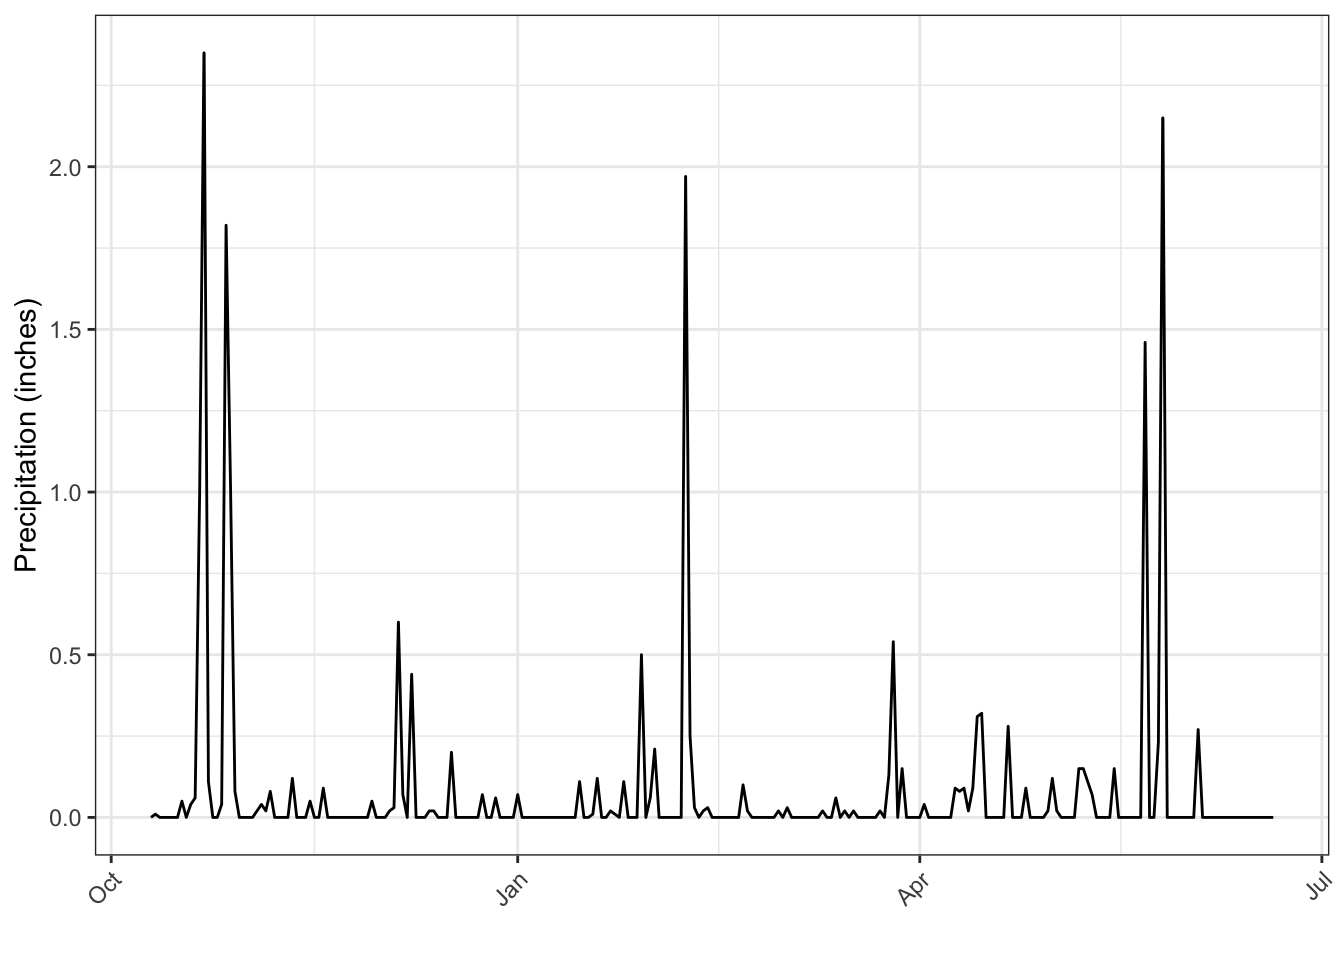
\includegraphics{jbb_reefs_files/figure-latex/unnamed-chunk-8-1.pdf}

\hypertarget{need-to-add}{%
\subsubsection{Need to add:}\label{need-to-add}}

\begin{itemize}
\tightlist
\item
  recruits
\item
  urchins
\end{itemize}

\hypertarget{fish}{%
\subsection{Fish}\label{fish}}

\begin{Shaded}
\begin{Highlighting}[]
\CommentTok{\# import and clean data}

\NormalTok{rf\_fish }\OtherTok{\textless{}{-}} \FunctionTok{read\_excel}\NormalTok{(}\FunctionTok{here}\NormalTok{(}\StringTok{"jumby\_baseline"}\NormalTok{, }\StringTok{"data"}\NormalTok{, }\StringTok{"JBB\_reefs.xlsx"}\NormalTok{), }\AttributeTok{sheet =} \StringTok{"fish"}\NormalTok{) }\SpecialCharTok{\%\textgreater{}\%}  
  \FunctionTok{clean\_names}\NormalTok{() }\SpecialCharTok{\%\textgreater{}\%}
  \FunctionTok{filter}\NormalTok{(}\SpecialCharTok{!}\FunctionTok{is.na}\NormalTok{(site)) }\SpecialCharTok{\%\textgreater{}\%} \CommentTok{\# remove any incomplete rows at the end of the data}
  \FunctionTok{mutate}\NormalTok{(}\AttributeTok{number =} \FunctionTok{if\_else}\NormalTok{(}\FunctionTok{is.na}\NormalTok{(number), }\DecValTok{1}\NormalTok{, number)) }\SpecialCharTok{\%\textgreater{}\%} \CommentTok{\# all entries with no number specified were single observations}
  \FunctionTok{uncount}\NormalTok{(number) }\SpecialCharTok{\%\textgreater{}\%} \CommentTok{\# expand to replicate rows if multiple fish were recorded to look at length distributions}
  \FunctionTok{mutate}\NormalTok{(}\AttributeTok{biomass =} \FunctionTok{as.numeric}\NormalTok{(biomass),}
         \AttributeTok{phase\_code =} \FunctionTok{tolower}\NormalTok{(phase),}
         \AttributeTok{phase =} \FunctionTok{case\_when}\NormalTok{(phase }\SpecialCharTok{==} \StringTok{"j"} \SpecialCharTok{\textasciitilde{}} \StringTok{"Juvenile"}\NormalTok{,}
\NormalTok{                           phase }\SpecialCharTok{==} \StringTok{"i"} \SpecialCharTok{\textasciitilde{}} \StringTok{"Initial"}\NormalTok{,}
\NormalTok{                           phase }\SpecialCharTok{==} \StringTok{"t"} \SpecialCharTok{\textasciitilde{}} \StringTok{"Terminal"}\NormalTok{),}
         \AttributeTok{family\_c =} \FunctionTok{if\_else}\NormalTok{(family }\SpecialCharTok{\%in\%} \FunctionTok{c}\NormalTok{(}\StringTok{"Scaridae"}\NormalTok{, }\StringTok{"Acanthuridae"}\NormalTok{, }\StringTok{"Haemulidae"}\NormalTok{, }\StringTok{"Serranidae"}\NormalTok{, }\StringTok{"Lutjanidae"}\NormalTok{, }\StringTok{"Balistidae"}\NormalTok{, }\StringTok{"Pomacentridae"}\NormalTok{), family, }\StringTok{"Other"}\NormalTok{)}
\NormalTok{         ) }\CommentTok{\# consolidating the number of families}
\end{Highlighting}
\end{Shaded}

\hypertarget{fish-biomass}{%
\subsubsection{Fish biomass}\label{fish-biomass}}

\hypertarget{total-biomass-at-each-site}{%
\paragraph{Total biomass at each
site}\label{total-biomass-at-each-site}}

\begin{itemize}
\tightlist
\item
  Regional averages are taken from Karr et al.~2015
\end{itemize}

\begin{Shaded}
\begin{Highlighting}[]
\CommentTok{\# calculating total biomass in each transect (sum) {-}\textgreater{} mean at each site}
\NormalTok{rf\_fish\_site }\OtherTok{\textless{}{-}}\NormalTok{ rf\_fish }\SpecialCharTok{\%\textgreater{}\%} 
  \FunctionTok{group\_by}\NormalTok{(site, transect) }\SpecialCharTok{\%\textgreater{}\%}
  \FunctionTok{summarize}\NormalTok{(}\AttributeTok{bm\_tot =} \FunctionTok{sum}\NormalTok{(biomass)}\SpecialCharTok{/}\DecValTok{1000}\SpecialCharTok{/}\DecValTok{120}\SpecialCharTok{*}\DecValTok{10000}\NormalTok{) }\SpecialCharTok{\%\textgreater{}\%} \CommentTok{\#kg/ha}
  \FunctionTok{group\_by}\NormalTok{(site) }\SpecialCharTok{\%\textgreater{}\%}
  \FunctionTok{summarize}\NormalTok{(}\AttributeTok{bm\_mean =} \FunctionTok{mean}\NormalTok{(bm\_tot),}
            \AttributeTok{bm\_se =} \FunctionTok{sd}\NormalTok{(bm\_tot)}\SpecialCharTok{/}\FunctionTok{sqrt}\NormalTok{(}\FunctionTok{n}\NormalTok{()))}
\end{Highlighting}
\end{Shaded}

\begin{Shaded}
\begin{Highlighting}[]
\CommentTok{\# graph}
\FunctionTok{ggplot}\NormalTok{(rf\_fish\_site, }\FunctionTok{aes}\NormalTok{(}\AttributeTok{x =}\NormalTok{ site, }\AttributeTok{y =}\NormalTok{ bm\_mean)) }\SpecialCharTok{+}
  \FunctionTok{geom\_col}\NormalTok{(}\AttributeTok{fill =} \StringTok{"cadetblue3"}\NormalTok{, }\AttributeTok{color =} \StringTok{"black"}\NormalTok{, }\AttributeTok{alpha =} \FloatTok{0.8}\NormalTok{) }\SpecialCharTok{+}
  \FunctionTok{geom\_errorbar}\NormalTok{(}\FunctionTok{aes}\NormalTok{(}\AttributeTok{ymin =}\NormalTok{ bm\_mean }\SpecialCharTok{{-}}\NormalTok{ bm\_se, }\AttributeTok{ymax =}\NormalTok{ bm\_mean }\SpecialCharTok{+}\NormalTok{ bm\_se), }\AttributeTok{width =}\NormalTok{ .}\DecValTok{2}\NormalTok{,}
                 \AttributeTok{position =} \FunctionTok{position\_dodge}\NormalTok{(.}\DecValTok{9}\NormalTok{)) }\SpecialCharTok{+}
  \FunctionTok{geom\_hline}\NormalTok{(}\AttributeTok{yintercept =} \DecValTok{1300}\NormalTok{, }\AttributeTok{linetype =} \StringTok{"dashed"}\NormalTok{, }\AttributeTok{color =} \StringTok{"black"}\NormalTok{) }\SpecialCharTok{+}
  \FunctionTok{annotate}\NormalTok{(}\StringTok{"text"}\NormalTok{, }\AttributeTok{x =} \FloatTok{5.5}\NormalTok{, }\AttributeTok{y =} \DecValTok{1350}\NormalTok{, }\AttributeTok{size =} \DecValTok{3}\NormalTok{, }\AttributeTok{hjust =} \DecValTok{1}\NormalTok{, }\AttributeTok{label=}\FunctionTok{c}\NormalTok{(}\StringTok{\textquotesingle{}Caribbean mean unfished biomass\textquotesingle{}}\NormalTok{)) }\SpecialCharTok{+}
  \FunctionTok{labs}\NormalTok{(}\AttributeTok{x =} \StringTok{""}\NormalTok{, }\AttributeTok{y =} \FunctionTok{expression}\NormalTok{(Total}\SpecialCharTok{\textasciitilde{}}\NormalTok{fish}\SpecialCharTok{\textasciitilde{}}\NormalTok{biomass}\SpecialCharTok{\textasciitilde{}}\NormalTok{(kg}\SpecialCharTok{\textasciitilde{}}\NormalTok{ha}\SpecialCharTok{\^{}{-}}\DecValTok{1}\NormalTok{))) }\SpecialCharTok{+}
  \FunctionTok{theme\_bw}\NormalTok{()}
\end{Highlighting}
\end{Shaded}

\includegraphics{jbb_reefs_files/figure-latex/unnamed-chunk-11-1.pdf}

\begin{Shaded}
\begin{Highlighting}[]
\FunctionTok{kable}\NormalTok{(rf\_fish\_site }\SpecialCharTok{\%\textgreater{}\%} \FunctionTok{select}\NormalTok{(site, bm\_mean, bm\_se))}
\end{Highlighting}
\end{Shaded}

\begin{longtable}[]{@{}lrr@{}}
\toprule()
site & bm\_mean & bm\_se \\
\midrule()
\endhead
Homer Point & 139.7707 & 25.35147 \\
Little Bird Island N & 156.1916 & 18.40841 \\
Little Bird Island W & 181.4903 & 47.19336 \\
Pasture Point & 349.4497 & 113.93810 \\
Pierce Shoals W & 186.7296 & 93.87824 \\
\bottomrule()
\end{longtable}

\hypertarget{biomass-by-site-and-family}{%
\subsubsection{Biomass by site and
family}\label{biomass-by-site-and-family}}

\begin{itemize}
\tightlist
\item
  Need to reorder to put ``other'' last
\item
  Are these good for families to feature?
\item
  Should I switch to common family names, or both?
\end{itemize}

\begin{Shaded}
\begin{Highlighting}[]
\NormalTok{rf\_fish\_fam\_site }\OtherTok{\textless{}{-}}\NormalTok{ rf\_fish }\SpecialCharTok{\%\textgreater{}\%} 
  \FunctionTok{expand}\NormalTok{(}\FunctionTok{nesting}\NormalTok{(site, transect), family\_c) }\SpecialCharTok{\%\textgreater{}\%}
  \FunctionTok{left\_join}\NormalTok{(rf\_fish }\SpecialCharTok{\%\textgreater{}\%}
      \FunctionTok{select}\NormalTok{(site, transect, family\_c, length, biomass)) }\SpecialCharTok{\%\textgreater{}\%}
  \FunctionTok{mutate}\NormalTok{(}\AttributeTok{biomass =} \FunctionTok{if\_else}\NormalTok{(}\FunctionTok{is.na}\NormalTok{(biomass), }\DecValTok{0}\NormalTok{, biomass)) }\SpecialCharTok{\%\textgreater{}\%}
  \FunctionTok{group\_by}\NormalTok{(site, transect, family\_c) }\SpecialCharTok{\%\textgreater{}\%}
  \FunctionTok{summarize}\NormalTok{(}\AttributeTok{bm\_tot =} \FunctionTok{sum}\NormalTok{(biomass)}\SpecialCharTok{/}\DecValTok{1000}\SpecialCharTok{/}\DecValTok{120}\SpecialCharTok{*}\DecValTok{10000}\NormalTok{) }\SpecialCharTok{\%\textgreater{}\%} \CommentTok{\#kg/ha}
  \FunctionTok{group\_by}\NormalTok{(site, family\_c) }\SpecialCharTok{\%\textgreater{}\%}
  \FunctionTok{summarize}\NormalTok{(}\AttributeTok{bm\_mean =} \FunctionTok{mean}\NormalTok{(bm\_tot),}
            \AttributeTok{bm\_se =} \FunctionTok{sd}\NormalTok{(bm\_tot)}\SpecialCharTok{/}\FunctionTok{sqrt}\NormalTok{(}\FunctionTok{n}\NormalTok{()))}
\end{Highlighting}
\end{Shaded}

\begin{Shaded}
\begin{Highlighting}[]
\CommentTok{\# graph}
\FunctionTok{ggplot}\NormalTok{(rf\_fish\_fam\_site, }\FunctionTok{aes}\NormalTok{(}\AttributeTok{x =}\NormalTok{ family\_c, }\AttributeTok{y =}\NormalTok{ bm\_mean)) }\SpecialCharTok{+}
  \FunctionTok{geom\_col}\NormalTok{(}\AttributeTok{fill =} \StringTok{"cadetblue3"}\NormalTok{, }\AttributeTok{color =} \StringTok{"black"}\NormalTok{, }\AttributeTok{alpha =} \FloatTok{0.9}\NormalTok{) }\SpecialCharTok{+}
  \FunctionTok{geom\_errorbar}\NormalTok{(}\FunctionTok{aes}\NormalTok{(}\AttributeTok{ymin =}\NormalTok{ bm\_mean }\SpecialCharTok{{-}}\NormalTok{ bm\_se, }\AttributeTok{ymax =}\NormalTok{ bm\_mean }\SpecialCharTok{+}\NormalTok{ bm\_se), }\AttributeTok{width =}\NormalTok{ .}\DecValTok{2}\NormalTok{,}
                 \AttributeTok{position =} \FunctionTok{position\_dodge}\NormalTok{(.}\DecValTok{9}\NormalTok{)) }\SpecialCharTok{+}
  \FunctionTok{facet\_wrap}\NormalTok{(. }\SpecialCharTok{\textasciitilde{}}\NormalTok{ site, }\AttributeTok{ncol =} \DecValTok{1}\NormalTok{) }\SpecialCharTok{+}
  \FunctionTok{labs}\NormalTok{(}\AttributeTok{x =} \StringTok{""}\NormalTok{, }\AttributeTok{y =} \FunctionTok{expression}\NormalTok{(Biomass}\SpecialCharTok{\textasciitilde{}}\NormalTok{(kg}\SpecialCharTok{\textasciitilde{}}\NormalTok{ha}\SpecialCharTok{\^{}{-}}\DecValTok{1}\NormalTok{))) }\SpecialCharTok{+}
  \FunctionTok{theme\_bw}\NormalTok{() }\SpecialCharTok{+}
  \FunctionTok{theme}\NormalTok{(}\AttributeTok{axis.text.x =} \FunctionTok{element\_text}\NormalTok{(}\AttributeTok{angle =} \DecValTok{45}\NormalTok{, }\AttributeTok{h =} \DecValTok{1}\NormalTok{))}
\end{Highlighting}
\end{Shaded}

\includegraphics{jbb_reefs_files/figure-latex/unnamed-chunk-13-1.pdf}

\begin{Shaded}
\begin{Highlighting}[]
\FunctionTok{kable}\NormalTok{(rf\_fish\_fam\_site }\SpecialCharTok{\%\textgreater{}\%} \FunctionTok{select}\NormalTok{(site, }\AttributeTok{family =}\NormalTok{ family\_c, bm\_mean, bm\_se))}
\end{Highlighting}
\end{Shaded}

\begin{longtable}[]{@{}llrr@{}}
\toprule()
site & family & bm\_mean & bm\_se \\
\midrule()
\endhead
Homer Point & Acanthuridae & 42.8908481 & 11.6572714 \\
Homer Point & Haemulidae & 0.5201659 & 0.5201659 \\
Homer Point & Lutjanidae & 6.3694441 & 6.3694441 \\
Homer Point & Other & 9.4074782 & 3.5483896 \\
Homer Point & Pomacentridae & 10.6749561 & 6.6431279 \\
Homer Point & Scaridae & 69.3588909 & 18.8969026 \\
Homer Point & Serranidae & 0.5488902 & 0.3430707 \\
Little Bird Island N & Acanthuridae & 35.9727390 & 7.7919239 \\
Little Bird Island N & Haemulidae & 6.5774270 & 3.3044487 \\
Little Bird Island N & Lutjanidae & 7.0848874 & 4.4216375 \\
Little Bird Island N & Other & 22.4505850 & 11.4622906 \\
Little Bird Island N & Pomacentridae & 10.3283883 & 4.0580768 \\
Little Bird Island N & Scaridae & 72.8543359 & 13.8844571 \\
Little Bird Island N & Serranidae & 0.9232343 & 0.4318075 \\
Little Bird Island W & Acanthuridae & 22.5085015 & 11.4739516 \\
Little Bird Island W & Haemulidae & 52.4258652 & 21.6198819 \\
Little Bird Island W & Lutjanidae & 15.0842021 & 3.4445261 \\
Little Bird Island W & Other & 30.4447117 & 8.4163357 \\
Little Bird Island W & Pomacentridae & 27.6073611 & 9.4573849 \\
Little Bird Island W & Scaridae & 31.8587441 & 6.6490737 \\
Little Bird Island W & Serranidae & 1.5608830 & 0.9406703 \\
Pasture Point & Acanthuridae & 47.4353959 & 14.0426872 \\
Pasture Point & Haemulidae & 128.4105447 & 114.2115388 \\
Pasture Point & Lutjanidae & 4.5480098 & 3.4988036 \\
Pasture Point & Other & 72.2111801 & 34.0993803 \\
Pasture Point & Pomacentridae & 10.1399444 & 6.6488481 \\
Pasture Point & Scaridae & 86.3867183 & 29.1056015 \\
Pasture Point & Serranidae & 0.3178841 & 0.3178841 \\
Pierce Shoals W & Acanthuridae & 45.1250994 & 28.8079159 \\
Pierce Shoals W & Haemulidae & 0.6092317 & 0.6092317 \\
Pierce Shoals W & Lutjanidae & 0.8799941 & 0.8799941 \\
Pierce Shoals W & Other & 9.8218799 & 3.2814828 \\
Pierce Shoals W & Pomacentridae & 15.4244093 & 1.8436711 \\
Pierce Shoals W & Scaridae & 113.1501279 & 66.3227768 \\
Pierce Shoals W & Serranidae & 1.7188308 & 1.2574469 \\
\bottomrule()
\end{longtable}

\hypertarget{herbivore-biomasses}{%
\subsubsection{Herbivore biomasses}\label{herbivore-biomasses}}

\hypertarget{scarid-biomass-by-site}{%
\paragraph{Scarid biomass by site}\label{scarid-biomass-by-site}}

\begin{itemize}
\item
  \begin{itemize}
  \tightlist
  \item
    Eastern Caribbean average parrotfish biomass for NTRs from Steneck
    et al.~2018 was \textasciitilde{} 1550 g/100m2, or 155 kg/ha. Note
    that this is potentially misleading because I'm sure a lot of these
    NTRs do experience some fishing. But mean fished parrotfish
    biomasses for the same region was \textasciitilde{} 750 g/100m2
  \end{itemize}
\end{itemize}

\begin{Shaded}
\begin{Highlighting}[]
\FunctionTok{ggplot}\NormalTok{(rf\_fish\_fam\_site }\SpecialCharTok{\%\textgreater{}\%}
        \FunctionTok{filter}\NormalTok{(family\_c }\SpecialCharTok{==} \StringTok{"Scaridae"}\NormalTok{),}
       \FunctionTok{aes}\NormalTok{(}\AttributeTok{x =}\NormalTok{ site, }\AttributeTok{y =}\NormalTok{ bm\_mean)) }\SpecialCharTok{+}
  \FunctionTok{geom\_col}\NormalTok{(}\AttributeTok{color =} \StringTok{"black"}\NormalTok{, }\AttributeTok{fill =} \StringTok{"cadetblue3"}\NormalTok{, }\AttributeTok{alpha =} \FloatTok{0.8}\NormalTok{, }\AttributeTok{stat =} \StringTok{"identity"}\NormalTok{, }\AttributeTok{position =} \FunctionTok{position\_dodge}\NormalTok{()) }\SpecialCharTok{+}
  \FunctionTok{geom\_errorbar}\NormalTok{(}\FunctionTok{aes}\NormalTok{(}\AttributeTok{ymin =}\NormalTok{ bm\_mean }\SpecialCharTok{{-}}\NormalTok{ bm\_se, }\AttributeTok{ymax =}\NormalTok{ bm\_mean }\SpecialCharTok{+}\NormalTok{ bm\_se), }\AttributeTok{width =}\NormalTok{ .}\DecValTok{2}\NormalTok{,}
                 \AttributeTok{position =} \FunctionTok{position\_dodge}\NormalTok{(.}\DecValTok{9}\NormalTok{)) }\SpecialCharTok{+}
  \FunctionTok{geom\_hline}\NormalTok{(}\AttributeTok{yintercept =} \DecValTok{155}\NormalTok{, }\AttributeTok{linetype =} \StringTok{"dashed"}\NormalTok{, }\AttributeTok{color =} \StringTok{"black"}\NormalTok{) }\SpecialCharTok{+}
  \FunctionTok{annotate}\NormalTok{(}\StringTok{"text"}\NormalTok{, }\AttributeTok{x =} \FloatTok{4.9}\NormalTok{, }\AttributeTok{y =} \DecValTok{165}\NormalTok{, }\AttributeTok{size =} \DecValTok{3}\NormalTok{, }\AttributeTok{hjust =} \DecValTok{1}\NormalTok{, }\AttributeTok{label=}\FunctionTok{c}\NormalTok{(}\StringTok{\textquotesingle{}Eastern Caribbean mean unfished biomass\textquotesingle{}}\NormalTok{)) }\SpecialCharTok{+}
  \FunctionTok{labs}\NormalTok{(}\AttributeTok{x =} \StringTok{""}\NormalTok{, }\AttributeTok{y =} \FunctionTok{expression}\NormalTok{(Parrotfish}\SpecialCharTok{\textasciitilde{}}\NormalTok{biomass}\SpecialCharTok{\textasciitilde{}}\NormalTok{(kg}\SpecialCharTok{\textasciitilde{}}\NormalTok{ha}\SpecialCharTok{\^{}{-}}\DecValTok{1}\NormalTok{))) }\SpecialCharTok{+}
  \FunctionTok{theme\_bw}\NormalTok{()}
\end{Highlighting}
\end{Shaded}

\includegraphics{jbb_reefs_files/figure-latex/unnamed-chunk-14-1.pdf}

\hypertarget{acanthurid-biomass-by-site}{%
\paragraph{Acanthurid biomass by
site}\label{acanthurid-biomass-by-site}}

\begin{Shaded}
\begin{Highlighting}[]
\FunctionTok{ggplot}\NormalTok{(rf\_fish\_fam\_site }\SpecialCharTok{\%\textgreater{}\%}
        \FunctionTok{filter}\NormalTok{(family\_c }\SpecialCharTok{==} \StringTok{"Acanthuridae"}\NormalTok{),}
       \FunctionTok{aes}\NormalTok{(}\AttributeTok{x =}\NormalTok{ site, }\AttributeTok{y =}\NormalTok{ bm\_mean)) }\SpecialCharTok{+}
  \FunctionTok{geom\_col}\NormalTok{(}\AttributeTok{color =} \StringTok{"black"}\NormalTok{, }\AttributeTok{fill =} \StringTok{"cadetblue3"}\NormalTok{, }\AttributeTok{alpha =} \FloatTok{0.8}\NormalTok{, }\AttributeTok{stat =} \StringTok{"identity"}\NormalTok{, }\AttributeTok{position =} \FunctionTok{position\_dodge}\NormalTok{()) }\SpecialCharTok{+}
  \FunctionTok{geom\_errorbar}\NormalTok{(}\FunctionTok{aes}\NormalTok{(}\AttributeTok{ymin =}\NormalTok{ bm\_mean }\SpecialCharTok{{-}}\NormalTok{ bm\_se, }\AttributeTok{ymax =}\NormalTok{ bm\_mean }\SpecialCharTok{+}\NormalTok{ bm\_se), }\AttributeTok{width =}\NormalTok{ .}\DecValTok{2}\NormalTok{,}
                 \AttributeTok{position =} \FunctionTok{position\_dodge}\NormalTok{(.}\DecValTok{9}\NormalTok{)) }\SpecialCharTok{+}
  \FunctionTok{labs}\NormalTok{(}\AttributeTok{x =} \StringTok{""}\NormalTok{, }\AttributeTok{y =} \FunctionTok{expression}\NormalTok{(Surgeonfish}\SpecialCharTok{\textasciitilde{}}\NormalTok{biomass}\SpecialCharTok{\textasciitilde{}}\NormalTok{(kg}\SpecialCharTok{\textasciitilde{}}\NormalTok{ha}\SpecialCharTok{\^{}{-}}\DecValTok{1}\NormalTok{))) }\SpecialCharTok{+}
  \FunctionTok{theme\_bw}\NormalTok{()}
\end{Highlighting}
\end{Shaded}

\includegraphics{jbb_reefs_files/figure-latex/unnamed-chunk-15-1.pdf}

\hypertarget{fish-lengths}{%
\subsubsection{Fish lengths}\label{fish-lengths}}

\begin{itemize}
\tightlist
\item
  These were calculated by taking the mean density of fish of each size
  at each size (averaged across transects). Because we have distribution
  data within each transect, we can't make density plots/violin plots
  straight from the raw data (i.e., some sites could have more
  transects)
\item
  Open to any suggestions about how we want to communicate size data!
\end{itemize}

\hypertarget{length-distributions-of-all-fish-by-site}{%
\paragraph{Length distributions of all fish by
site}\label{length-distributions-of-all-fish-by-site}}

\begin{Shaded}
\begin{Highlighting}[]
\NormalTok{rf\_fish\_length }\OtherTok{\textless{}{-}}\NormalTok{ rf\_fish }\SpecialCharTok{\%\textgreater{}\%}
  \FunctionTok{expand}\NormalTok{(}\FunctionTok{nesting}\NormalTok{(site, transect), length) }\SpecialCharTok{\%\textgreater{}\%}
  \FunctionTok{left\_join}\NormalTok{(rf\_fish }\SpecialCharTok{\%\textgreater{}\%}
        \FunctionTok{group\_by}\NormalTok{(site, transect, length) }\SpecialCharTok{\%\textgreater{}\%}
        \FunctionTok{summarize}\NormalTok{(}\AttributeTok{count =} \FunctionTok{n}\NormalTok{())) }\SpecialCharTok{\%\textgreater{}\%}
  \FunctionTok{mutate}\NormalTok{(}\AttributeTok{count =} \FunctionTok{as.numeric}\NormalTok{(count),}
         \AttributeTok{count =} \FunctionTok{if\_else}\NormalTok{(}\FunctionTok{is.na}\NormalTok{(count), }\DecValTok{0}\NormalTok{, count),}
         \AttributeTok{density =}\NormalTok{ count}\SpecialCharTok{/}\DecValTok{120}\NormalTok{) }\SpecialCharTok{\%\textgreater{}\%} \CommentTok{\# indv./m2}
  \FunctionTok{group\_by}\NormalTok{(site, length) }\SpecialCharTok{\%\textgreater{}\%}
  \FunctionTok{summarize}\NormalTok{(}\AttributeTok{density\_mean =} \FunctionTok{mean}\NormalTok{(density),}
            \AttributeTok{density\_se =} \FunctionTok{sd}\NormalTok{(density)}\SpecialCharTok{/}\FunctionTok{sqrt}\NormalTok{(}\FunctionTok{n}\NormalTok{()))}

\FunctionTok{ggplot}\NormalTok{(rf\_fish\_length, }\FunctionTok{aes}\NormalTok{(}\AttributeTok{x =}\NormalTok{ length, }\AttributeTok{y =}\NormalTok{ density\_mean)) }\SpecialCharTok{+}
  \FunctionTok{geom\_col}\NormalTok{(}\AttributeTok{fill =} \StringTok{"deepskyblue4"}\NormalTok{, }\AttributeTok{alpha =} \FloatTok{0.9}\NormalTok{, }\AttributeTok{color =} \StringTok{"black"}\NormalTok{) }\SpecialCharTok{+}
  \FunctionTok{facet\_wrap}\NormalTok{(. }\SpecialCharTok{\textasciitilde{}}\NormalTok{ site) }\SpecialCharTok{+}
  \FunctionTok{labs}\NormalTok{(}\AttributeTok{x =} \StringTok{"Fish length (cm)"}\NormalTok{, }\AttributeTok{y =} \FunctionTok{expression}\NormalTok{(Density}\SpecialCharTok{\textasciitilde{}}\NormalTok{(indv.}\SpecialCharTok{\textasciitilde{}}\NormalTok{m}\SpecialCharTok{\^{}{-}}\DecValTok{2}\NormalTok{))) }\SpecialCharTok{+}
  \FunctionTok{theme\_bw}\NormalTok{()}
\end{Highlighting}
\end{Shaded}

\includegraphics{jbb_reefs_files/figure-latex/unnamed-chunk-16-1.pdf}

\hypertarget{length-distributions-of-scarids-at-each-site}{%
\paragraph{Length distributions of scarids at each
site}\label{length-distributions-of-scarids-at-each-site}}

\begin{Shaded}
\begin{Highlighting}[]
\NormalTok{rf\_fish\_length\_scarids }\OtherTok{\textless{}{-}}\NormalTok{ rf\_fish }\SpecialCharTok{\%\textgreater{}\%}
  \FunctionTok{expand}\NormalTok{(}\FunctionTok{nesting}\NormalTok{(site, transect), length) }\SpecialCharTok{\%\textgreater{}\%}
  \FunctionTok{left\_join}\NormalTok{(rf\_fish }\SpecialCharTok{\%\textgreater{}\%}
        \FunctionTok{filter}\NormalTok{(family }\SpecialCharTok{==} \StringTok{"Scaridae"}\NormalTok{) }\SpecialCharTok{\%\textgreater{}\%}
        \FunctionTok{group\_by}\NormalTok{(site, transect, length) }\SpecialCharTok{\%\textgreater{}\%}
        \FunctionTok{summarize}\NormalTok{(}\AttributeTok{count =} \FunctionTok{n}\NormalTok{())) }\SpecialCharTok{\%\textgreater{}\%}
  \FunctionTok{mutate}\NormalTok{(}\AttributeTok{count =} \FunctionTok{as.numeric}\NormalTok{(count),}
         \AttributeTok{count =} \FunctionTok{if\_else}\NormalTok{(}\FunctionTok{is.na}\NormalTok{(count), }\DecValTok{0}\NormalTok{, count),}
         \AttributeTok{density =}\NormalTok{ count}\SpecialCharTok{/}\DecValTok{120}\NormalTok{) }\SpecialCharTok{\%\textgreater{}\%} \CommentTok{\# invd/m2}
  \FunctionTok{group\_by}\NormalTok{(site, length) }\SpecialCharTok{\%\textgreater{}\%}
  \FunctionTok{summarize}\NormalTok{(}\AttributeTok{density\_mean =} \FunctionTok{mean}\NormalTok{(density),}
            \AttributeTok{density\_se =} \FunctionTok{sd}\NormalTok{(density)}\SpecialCharTok{/}\FunctionTok{sqrt}\NormalTok{(}\FunctionTok{n}\NormalTok{()))}

\FunctionTok{ggplot}\NormalTok{(rf\_fish\_length\_scarids, }\FunctionTok{aes}\NormalTok{(}\AttributeTok{x =}\NormalTok{ length, }\AttributeTok{y =}\NormalTok{ density\_mean)) }\SpecialCharTok{+}
  \FunctionTok{geom\_col}\NormalTok{(}\AttributeTok{fill =} \StringTok{"deepskyblue4"}\NormalTok{, }\AttributeTok{alpha =} \FloatTok{0.9}\NormalTok{, }\AttributeTok{color =} \StringTok{"black"}\NormalTok{) }\SpecialCharTok{+}
  \FunctionTok{facet\_wrap}\NormalTok{(. }\SpecialCharTok{\textasciitilde{}}\NormalTok{ site) }\SpecialCharTok{+}
  \FunctionTok{labs}\NormalTok{(}\AttributeTok{x =} \StringTok{"Fish length (cm)"}\NormalTok{, }\AttributeTok{y =} \FunctionTok{expression}\NormalTok{(Scarid}\SpecialCharTok{\textasciitilde{}}\NormalTok{density}\SpecialCharTok{\textasciitilde{}}\NormalTok{(indv.}\SpecialCharTok{\textasciitilde{}}\NormalTok{m}\SpecialCharTok{\^{}{-}}\DecValTok{2}\NormalTok{))) }\SpecialCharTok{+}
  \FunctionTok{theme\_bw}\NormalTok{()}
\end{Highlighting}
\end{Shaded}

\includegraphics{jbb_reefs_files/figure-latex/unnamed-chunk-17-1.pdf}

\end{document}
